\section{Fixed NPF regime}
\textbf{A New semi-idealised regime with fixed NPF(Resolving Gap II):} \Cref{tb:dynamics} shows the dynamics of GD for infinitesimal step-size (expressed in the form of coupled ordinary differential equations) in three regimes namely i) \emph{standard regime}, in  which practical DNNs operate, ii) \emph{fixed NTK regime}, an idealised regime which has been studied in recent works and iii) \emph{fixed NPF regime}, a new, semi-ideal regime which we introduce and study in this paper. In the standard regime, all the underlying quantities namely the weights, the NPFs, the NPVs and the error changes with time. In the fixed NTK regime, owing to the infinite width, while the weights and activations stay close to initialisation, and the cumulative effect drives the output to the required values, thereby reducing the training error. The fixed NPF regime, holds for any finite $w$, and here, we forcefully \emph{turn-off} feature learning, i.e. let the feature gradient $\psi^{\phi}_{x,\Theta}=0$. In order to do this, we hold the gates and hence the NPFs in a separate gating network and the NPVs in a different network called value network. By letting the parameters of the gating network non-trainable, we can force $\psi^{\phi}_{x,\Theta}$ to be $0$. Note that, in the limit of infinite width, the fixed NPF regime transitions to the fixed NTK regime. 
\FloatBarrier
\begin{table}[h]\centering
\resizebox{\columnwidth}{!}{
\begin{tabular}{| l | l | l |}\hline
Standard (finite $w$) &Fixed NTK ($w\ra\infty$) & Fixed NPK (finite $w$)\\\hline
$\dot{\Theta}_t=-\sum_{s=1}^n \psi_{x,t}e_t(s)$ &$\dot{\Theta}_t\ra 0$ &$\dot{\Theta}_t=-\sum_{s=1}^n \psi^v_{x,t}e_t(s)$ \\\hline
$\dot{\phi}_{x_s,t}(p)=x(\I_0(p))\sum_{\theta\in\Theta}\partial_{\theta}A_t(x_s,p)\dot{\theta}_t$ &$\dot{\phi}_{x_s,t}(p)\ra 0$ &$\dot{\phi}_{x_s,t}(p)=0$\\\hline
$\dot{v}_t(p)=\sum_{\theta\in\Theta}\partial_{\theta}v_t(p)\dot{\theta}_t$ &$\dot{v}_t(p)\ra 0$ &$\dot{v}_t(p)=\sum_{\theta\in\Theta}\partial_{\theta}v_t(p)\dot{\theta}_t$\\\hline
$\dot{e}_t=-(K^v_t+K^{\phi}_t+K^{cross}_{t})e_t$ &$\dot{e}_t=-K^{(d)}e_t$ &$\dot{e}_t=-K^v_te_t$\\\hline
\end{tabular}
}
\caption{Dynamics in various regimes. Here $p\in[P], s\in[n]$.}
\label{tb:dynamics}
\end{table}
We first show that fixed NPFs can be trained and they also generalise \Cref{th:main}. We then

\begin{table}[h] 
\begin{minipage}{0.75\columnwidth}
\resizebox{\columnwidth}{!}{
\begin{tabular}{|l|l|l|}\hline
Layer& Gating Network (NPF)&Value Network (NPV)\\\hline 
Input & $z_{x,\Tg_t}(0)=x$ &$z_{x,\Theta_t}(0)=x$ \\\hline
Activation & $q_{x,\Tg_t}(l)={\Tg_t(l)}^\top z_{x,\Tg_t}(l-1)$& $q_{x,\Theta_t}(l)={\Theta_t(l)}^\top z_{x,\Theta_t}(l-1)$\\\hline
Hidden &$z_{x,\Tg_t}(l)=q_{x,\Tg_t}(l)\odot G_{x,\Tg_t}(l)$& $z_{x,\Theta_t}(l)=q_{x,\Theta_t}(l)\odot G_{x,t}(l)$ \\\hline
Output & None &$\hat{y}_t(x)={\Theta_t(d)}^\top z_{x,\Theta_t}(d-1)$\\\hline
\multicolumn{3}{|l|}{Gating Values}\\\hline
\end{tabular}
}
\end{minipage}
\begin{minipage}{0.24\columnwidth}
\resizebox{\columnwidth}{!}{
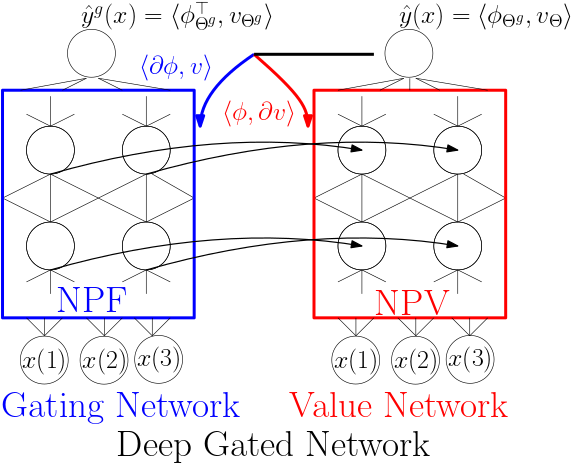
\includegraphics[scale=0.5]{figs/nntwin-blck.png}
}
\end{minipage}
\caption{}
\label{tb:dgn}
\end{table}
\begin{comment}
\begin{table}[h]
\centering
\resizebox{\columnwidth}{!}{
\begin{tabular}{|c|c|c|c|}\hline
		&Gate&Activation&$\dot{\chi}$\\\hline
Prior&$G_R(q)=\mathbbm{1}_{\{q>0\}}$& $\begin{aligned}\chi_{R}(q)&=q\cdot\mathbbm{1}_{\{q>0\}}\\ \chi_{SP}(q)&=\frac{1}{\beta}\log(1+\exp(\beta q))\end{aligned}$&$\begin{aligned}\dot{\chi_{R}}(q)&: \text{Heaviside step function} \\ \dot{\chi}_{SP}(q)&=\frac{1}{1+\exp(-\beta q)}\end{aligned}$ \\\hline
Ours &$G_{SR}(q)=\frac{1}{1+\exp(-\beta q)}$ &$\chi_{SR}(q)=q\cdot G_{SR}(q)$& $\dot{\chi}_{SR}(q)=\dot{\chi}_{SP}(q)+\underbrace{\dot{G}_{SR}(q)}_{\text{Gate Dynamics}}$\\\hline
\end{tabular}
}
\caption{A comparison of prior work and our paper. Here subscripts $R$, $SR$ and $SP$ stand for ReLU, soft-ReLU and softplus respectively.}
\label{tb:compare}
\end{table}
\begin{table}[h]
\centering
\resizebox{\columnwidth}{!}{
\begin{tabular}{|c|c|c|c|c|}\hline
		&Output&NTF&$NTK$ &$\dot{\Sigma}^{(l+1)}(s,s')$\\\hline
Prior&\shortstack{$\hat{y}_{\Theta}(x)$\\layer-by-layer} &$\psi_{x,\Theta}=\left(\partial_{\theta}\hat{y}_{\Theta}(x),\theta\in\Theta\right)$& $K_{\Theta}(x,x')=\ip{\psi_{x,\Theta},\psi_{x',\Theta}}$ & $\dot{\chi}_{SP}(q)\dot{\chi}_{SP}(q')$ \\\hline
Ours& $\hat{y}_{\Theta}(x)=\ip{\phi_{x,\Theta},v_{\Theta}}$ & $\begin{aligned}\psi_{x,\Theta}&=\psi^v_{x,\Theta}+\psi^{\phi}_{x,\Theta}\\\psi^v_{x,\Theta}&=\left(\ip{\phi_{x,\Theta}, \partial_{\theta} v_{\Theta}},\theta\in\Theta\right) \\ \psi^{\phi}_{x,\Theta}&=\left(\ip{\partial_{\theta}\phi_{x,\Theta}, v_{\Theta}},\theta\in\Theta\right)\end{aligned}$ &$\begin{aligned} K_{\Theta}(x,x')=\langle \psi^v_{x,\Theta}+\psi^{\phi}_{x,\Theta},\\ \psi^v_{x',\Theta}+\psi^{\phi}_{x',\Theta}\rangle\end{aligned}$ & $\begin{aligned}\left(\dot{\chi}_{SP}(q)+\dot{G}_{SR}(q)\right)\cdot\\\left(\dot{\chi}_{SP}(q')+\dot{G}_{SR}(q')\right)\end{aligned}$ \\\hline

\end{tabular}
}
\caption{A comparison of prior work and our paper. Here subscripts $R$, $SR$ and $SP$ stand for ReLU, soft-ReLU and softplus respectively.}
\label{tb:compare}
\end{table}
\end{comment}
%$\begin{aligned}&\text{Learning}\\ &\text{Regime} \end{aligned}$ 